% This LaTeX document needs to be compiled with XeLaTeX.
\documentclass[10pt]{article}
\usepackage[utf8]{inputenc}
\usepackage{graphicx}
\usepackage[export]{adjustbox}
\graphicspath{ {./images/} }
\usepackage{amsmath}
\usepackage{amsfonts}
\usepackage{amssymb}
\usepackage[version=4]{mhchem}
\usepackage{stmaryrd}
\usepackage{multirow}
\usepackage[fallback]{xeCJK}
\usepackage{polyglossia}
\usepackage{fontspec}
\setCJKmainfont{Noto Serif CJK TC}

\setmainlanguage{polish}
\setmainfont{CMU Serif}

\title{Czas pracy 180 minut }

\author{}
\date{}


\begin{document}
\maketitle
\begin{center}
\begin{tabular}{|c|c}
\hline
\begin{tabular}{c}
Miejsce \\
na naklejkę \\
\end{tabular} &  \\
\hline
EGZAMIN MATURALNY & MMA-R1\_1P-092 \\
\hline
Z MATEMATYKI & ROK 2009 \\
POZIOM ROZSZERZONY &  \\
\hline
\end{tabular}
\end{center}

\section*{Instrukcja dla zdającego}
\begin{enumerate}
  \item Sprawdź, czy arkusz egzaminacyjny zawiera 16 stron (zadania 1-11). Ewentualny brak zgłoś przewodniczacemu zespołu nadzorującego egzamin.
  \item Rozwiązania zadań i odpowiedzi zamieść w miejscu na to przeznaczonym.
  \item W rozwiązaniach zadań przedstaw tok rozumowania prowadzacy do ostatecznego wyniku.
  \item Pisz czytelnie. Używaj długopisu/pióra tylko z czarnym tuszem/atramentem.
  \item Nie używaj korektora, a błędne zapisy przekreśl.
  \item Pamiętaj, że zapisy w brudnopisie nie podlegają ocenie.
  \item Obok każdego zadania podana jest maksymalna liczba punktów, którą możesz uzyskać za jego poprawne rozwiązanie.
  \item Możesz korzystać z zestawu wzorów matematycznych, cyrkla i linijki oraz kalkulatora.
  \item Na karcie odpowiedzi wpisz swoją datę urodzenia i PESEL. Nie wpisuj żadnych znaków w części przeznaczonej dla egzaminatora.\\

\includegraphics[max width=\textwidth, center]{2024_11_21_8bf32a7596bd08ca7a9fg-01(2)}
\end{enumerate}

Za rozwiązanie wszystkich zadań można otrzymać\\
łącznie\\
50 punktów\\
Życzymy powodzenia!

Wypelnia zdający\\
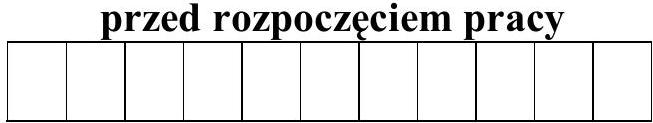
\includegraphics[max width=\textwidth, center]{2024_11_21_8bf32a7596bd08ca7a9fg-01(1)}

PESEL ZDAJĄCEGO\\

\includegraphics[max width=\textwidth, center]{2024_11_21_8bf32a7596bd08ca7a9fg-01}

\section*{Zadanie 1. (4 pkt)}
Funkcja liniowa \(f\) określona jest wzorem \(f(x)=a x+b\) dla \(x \in R\).\\
a) Dla \(a=2008\) i \(b=2009\) zbadaj, czy do wykresu tej funkcji należy punkt \(P=\left(2009,2009^{2}\right)\).\\
b) Narysuj w układzie współrzędnych zbiór

\[
A=\left\{(x, y): x \in\langle-1,3\rangle \text { i } y=-\frac{1}{2} x+b \text { i } b \in\langle-2,1\rangle\right\} .
\]

\begin{center}

\includegraphics[max width=\textwidth]{2024_11_21_8bf32a7596bd08ca7a9fg-02}
\end{center}

\begin{center}
\begin{tabular}{|c|l|c|c|c|c|}
\hline
\multirow{2}{*}{\begin{tabular}{c}
Wypelnia \\
egzaminator! \\
\end{tabular}} & Nr czynności & 1.1. & 1.2. & 1.3. & 1.4. \\
\cline{2-6} & Maks. liczba pkt & 1 & 1 & 1 & 1 \\
\cline{2-6} & Uzyskana liczba pkt &  &  &  &  \\
\hline
\end{tabular}
\end{center}

Zadanie 2. (4 pkt)\\
Przy dzieleniu wielomianu \(W(x)\) przez dwumian \((x-1)\) otrzymujemy iloraz \(Q(x)=8 x^{2}+4 x-14\) oraz resztę \(R(x)=-5\). Oblicz pierwiastki wielomianu \(W(x)\).

\begin{center}
\begin{tabular}{|c|c|c|c|c|c|c|c|c|c|c|c|c|c|c|c|c|c|c|c|c|c|c|c|c|}
\hline
 &  &  &  &  &  &  &  &  &  &  &  &  &  &  &  &  &  &  &  &  &  &  &  &  \\
\hline
 &  &  &  &  &  &  &  &  &  &  &  &  &  &  &  &  &  &  &  &  &  &  &  &  \\
\hline
 &  &  &  &  &  &  &  &  &  &  &  &  &  &  &  &  &  &  &  &  &  &  &  &  \\
\hline
 &  &  &  &  &  &  &  &  &  &  &  &  &  &  &  &  &  &  &  &  &  &  &  &  \\
\hline
 &  &  &  &  &  &  &  &  &  &  &  &  &  &  &  &  &  &  &  &  &  &  &  &  \\
\hline
 &  &  &  &  &  &  &  &  &  &  &  &  &  &  &  &  &  &  &  &  &  &  &  &  \\
\hline
 &  &  &  &  &  &  &  &  &  &  &  &  &  &  &  &  &  &  &  &  &  &  &  &  \\
\hline
 &  &  &  &  &  &  &  &  &  &  &  &  &  &  &  &  &  &  &  &  &  &  &  &  \\
\hline
 &  &  &  &  &  &  &  &  &  &  &  &  &  &  &  &  &  &  &  &  &  &  &  &  \\
\hline
 &  &  &  &  &  &  &  &  &  &  &  &  &  &  &  &  &  &  &  &  &  &  &  &  \\
\hline
 &  &  &  &  &  &  &  &  &  &  &  &  &  &  &  &  &  &  &  &  &  &  &  &  \\
\hline
 &  &  &  &  &  &  &  &  &  &  &  &  &  &  &  &  &  &  &  &  &  &  &  &  \\
\hline
 &  &  &  &  &  &  &  &  &  &  &  &  &  &  &  &  &  &  &  &  &  &  &  &  \\
\hline
 &  &  &  &  &  &  &  &  &  &  &  &  &  &  &  &  &  &  &  &  &  &  &  &  \\
\hline
 &  &  &  &  &  &  &  &  &  &  &  &  &  &  &  &  &  &  &  &  &  &  &  &  \\
\hline
 &  &  &  &  &  &  &  &  &  &  &  &  &  &  &  &  &  &  &  &  &  &  &  &  \\
\hline
 &  &  &  &  &  &  &  &  &  &  &  &  &  &  &  &  &  &  &  &  &  &  &  &  \\
\hline
 &  &  &  &  &  &  &  &  &  &  &  &  &  &  &  &  &  &  &  &  &  &  &  &  \\
\hline
 &  &  &  &  &  &  &  &  &  &  &  &  &  &  &  &  &  &  &  &  &  &  &  &  \\
\hline
 &  &  &  &  &  &  &  &  &  &  &  &  &  &  &  &  &  &  &  &  &  &  &  &  \\
\hline
 &  &  &  &  &  &  &  &  &  &  &  &  &  &  &  &  &  &  &  &  &  &  &  &  \\
\hline
 &  &  &  &  &  &  &  &  &  &  &  &  &  &  &  &  &  &  &  &  &  &  &  &  \\
\hline
 &  &  &  &  &  &  &  &  &  &  &  &  &  &  &  &  &  &  &  &  &  &  &  &  \\
\hline
 &  &  &  &  &  &  &  &  &  &  &  &  &  &  &  &  &  &  &  &  &  &  &  &  \\
\hline
 &  &  &  &  &  &  &  &  &  &  &  &  &  &  &  &  &  &  &  &  &  &  &  &  \\
\hline
 &  &  &  &  &  &  &  &  &  &  &  &  &  &  &  &  &  &  &  &  &  &  &  &  \\
\hline
 &  &  &  &  &  &  &  &  &  &  &  &  &  &  &  &  &  &  &  &  &  &  &  &  \\
\hline
 &  &  &  &  &  &  &  &  &  &  &  &  &  &  &  &  &  &  &  &  &  &  &  &  \\
\hline
 &  &  &  &  &  &  &  &  &  &  &  &  &  &  &  &  &  &  &  &  &  &  &  &  \\
\hline
 & \textbackslash  &  &  &  &  &  &  &  &  &  &  &  &  &  &  &  &  &  &  &  &  &  &  &  \\
\hline
 & \(\square\) &  &  &  &  &  &  &  &  &  &  &  &  &  &  &  &  &  &  &  &  &  &  &  \\
\hline
 &  &  &  &  &  &  &  &  &  &  &  &  &  &  &  &  &  &  &  &  &  &  &  &  \\
\hline
 &  &  &  &  &  &  &  &  &  &  &  &  &  &  &  &  &  &  &  &  &  &  &  &  \\
\hline
 &  &  &  &  &  &  &  &  &  &  &  &  &  &  &  &  &  &  &  &  &  &  &  &  \\
\hline
 &  &  &  &  &  &  &  &  &  &  &  &  &  &  &  &  &  &  &  &  &  &  &  &  \\
\hline
 & , &  &  &  &  &  &  &  &  &  &  &  &  &  &  &  &  &  &  &  &  &  &  &  \\
\hline
 &  &  &  &  &  &  &  &  &  &  &  &  &  &  &  &  &  &  &  &  &  &  &  &  \\
\hline
 &  &  &  &  &  &  &  &  &  &  &  &  &  &  &  &  &  &  &  &  &  &  &  &  \\
\hline
 & 到 &  &  &  &  &  &  &  &  &  &  &  &  &  &  &  &  &  &  &  &  &  &  &  \\
\hline
 & - &  &  &  &  &  &  &  &  &  &  &  &  &  &  &  &  &  &  &  &  &  &  &  \\
\hline
 &  &  &  &  &  &  &  &  &  &  &  &  &  &  &  &  &  &  &  &  &  &  &  &  \\
\hline
 & 到 &  &  &  &  &  &  &  &  &  &  &  &  &  &  &  &  &  &  &  &  &  &  &  \\
\hline
 &  &  &  &  &  &  &  &  &  &  &  &  &  &  &  &  &  &  &  &  &  &  &  &  \\
\hline
 &  &  &  &  &  &  &  &  &  &  &  &  &  &  &  &  &  &  &  &  &  &  &  &  \\
\hline
\end{tabular}
\end{center}

\begin{center}
\begin{tabular}{|c|l|c|c|c|c|}
\hline
\multirow{2}{*}{\begin{tabular}{c}
Wypelnia \\
egzaminator! \\
\end{tabular}} & Nr czynności & 2.1. & 2.2. & 2.3. & 2.4. \\
\cline { 2 - 6 }
 & Maks. liczba pkt & 1 & 1 & 1 & 1 \\
\cline { 2 - 6 }
 & Uzyskana liczba pkt &  &  &  &  \\
\hline
\end{tabular}
\end{center}

\section*{Zadanie 3. (4 pkt)}
Na rysunku przedstawiony jest wykres funkcji wykładniczej \(f(x)=a^{x}\) dla \(x \in R\).\\
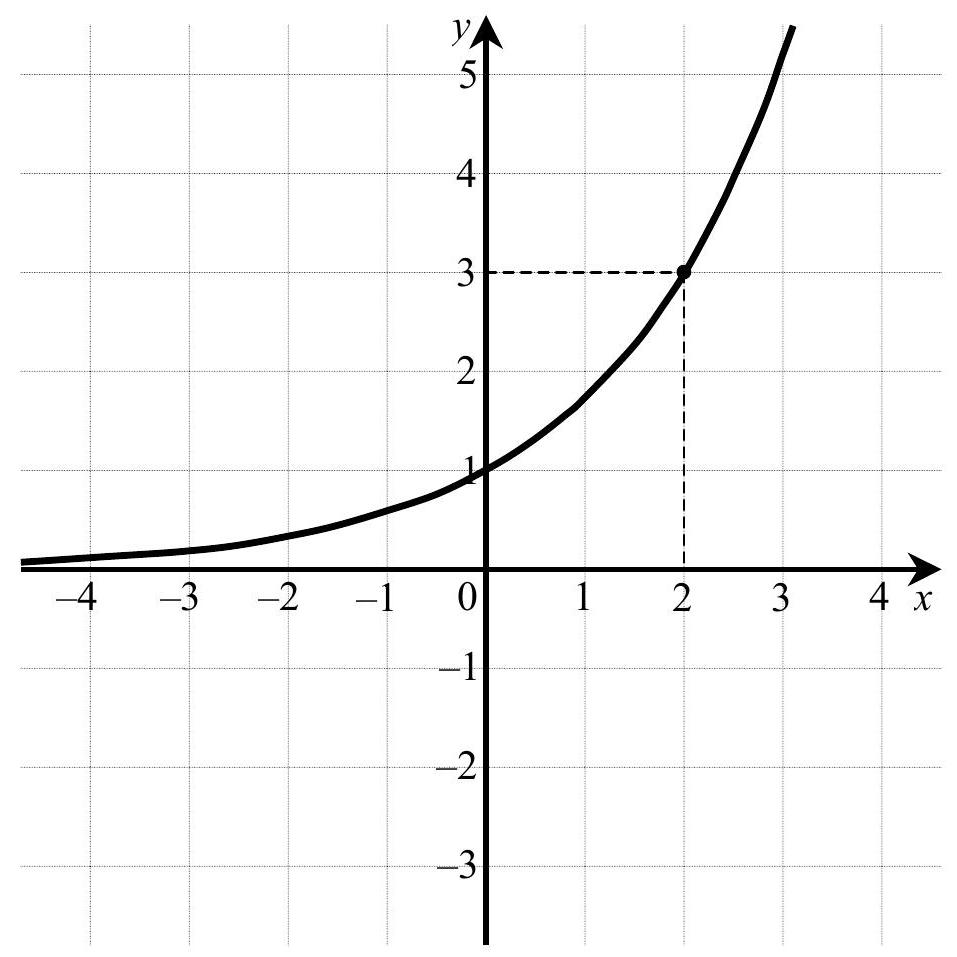
\includegraphics[max width=\textwidth, center]{2024_11_21_8bf32a7596bd08ca7a9fg-04}\\
a) Oblicz \(a\).\\
b) Narysuj wykres funkcji \(g(x)=|f(x)-2|\) i podaj wszystkie wartości parametru \(m \in R\), dla których równanie \(g(x)=m\) ma dokładnie jedno rozwiązanie.\\

\includegraphics[max width=\textwidth, center]{2024_11_21_8bf32a7596bd08ca7a9fg-04(1)}\\

\includegraphics[max width=\textwidth, center]{2024_11_21_8bf32a7596bd08ca7a9fg-05}

\begin{center}
\begin{tabular}{|c|l|c|c|c|c|}
\hline
\multirow{2}{*}{\begin{tabular}{c}
Wypetnia \\
egzaminator! \\
\end{tabular}} & Nr czynności & 3.1. & 3.2. & 3.3. & 3.4. \\
\cline { 2 - 6 }
 & Maks. liczba pkt & 1 & 1 & 1 & 1 \\
\cline { 2 - 6 }
 & Uzyskana liczba pkt &  &  &  &  \\
\hline
\end{tabular}
\end{center}

\section*{Zadanie 4. (5 pkt)}
W skarbcu królewskim było \(k\) monet. Pierwszego dnia rano skarbnik dorzucił 25 monet, a każdego następnego ranka dorzucał o 2 monety więcej niż dnia poprzedniego. Jednocześnie ze skarbca król zabierał w południe każdego dnia 50 monet. Oblicz najmniejszą liczbę \(k\), dla której w każdym dniu w skarbcu była co najmniej jedna moneta, a następnie dla tej wartości \(k\) oblicz, w którym dniu w skarbcu była najmniejsza liczba monet.\\

\includegraphics[max width=\textwidth, center]{2024_11_21_8bf32a7596bd08ca7a9fg-06}

\section*{Zadanie 5. (3 pkt)}
Wykaż, że jeżeli \(A=3^{4 \sqrt{2}+2}\) i \(B=3^{2 \sqrt{2}+3}\), to \(B=9 \sqrt{A}\).\\

\includegraphics[max width=\textwidth, center]{2024_11_21_8bf32a7596bd08ca7a9fg-07}

\begin{center}
\begin{tabular}{|c|l|c|c|c|}
\hline
\multirow{2}{*}{\begin{tabular}{c}
Wypelnia \\
egzaminator! \\
\end{tabular}} & Nr czynności & 5.1. & 5.2. & 5.3. \\
\cline { 2 - 5 }
 & Maks. liczba pkt & 1 & 1 & 1 \\
\cline { 2 - 5 }
 & Uzyskana liczba pkt &  &  &  \\
\hline
\end{tabular}
\end{center}

\section*{Zadanie 6. (5 pkt)}
Wyznacz dziedzinę funkcji \(f(x)=\log _{2 \cos x}\left(9-x^{2}\right)\) i zapisz ją w postaci sumy przedziałów liczbowych.\\

\includegraphics[max width=\textwidth, center]{2024_11_21_8bf32a7596bd08ca7a9fg-08}

\begin{center}
\begin{tabular}{|c|l|c|c|c|c|c|}
\hline
\multirow{2}{*}{\begin{tabular}{c}
Wypełnia \\
egzaminator! \\
\end{tabular}} & Nr czynności & 6.1. & 6.2. & 6.3. & 6.4. & 6.5. \\
\cline { 2 - 7 }
 & Maks. liczba pkt & 1 & 1 & 1 & 1 & 1 \\
\cline { 2 - 7 }
 & Uzyskana liczba pkt &  &  &  &  &  \\
\hline
\end{tabular}
\end{center}

\section*{Zadanie 7. (6 pkt)}
Ciag \((x-3, x+3,6 x+2, \ldots)\) jest nieskończonym ciagiem geometrycznym o wyrazach dodatnich. Oblicz iloraz tego ciagu i uzasadnij, że \(\frac{S_{19}}{S_{20}}<\frac{1}{4}\), gdzie \(S_{n}\) oznacza sumę \(n\) początkowych wyrazów tego ciagu.\\

\includegraphics[max width=\textwidth, center]{2024_11_21_8bf32a7596bd08ca7a9fg-09}

\begin{center}
\begin{tabular}{|c|l|c|c|c|c|c|c|}
\hline
\multirow{2}{*}{\begin{tabular}{c}
Wypełnia \\
egzaminator! \\
\end{tabular}} & Nr czynności & 7.1. & 7.2. & 7.3. & 7.4. & 7.5. & 7.6. \\
\cline { 2 - 8 }
 & Maks. liczba pkt & 1 & 1 & 1 & 1 & 1 & 1 \\
\cline { 2 - 8 }
 & Uzyskana liczba pkt &  &  &  &  &  &  \\
\hline
\end{tabular}
\end{center}

\section*{Zadanie 8. (4 pkt)}
Dwa okręgi o środkach \(A\) i \(B\) są styczne zewnętrznie i każdy z nich jest jednocześnie styczny do ramion tego samego kąta prostego (patrz rysunek). Udowodnij, że stosunek promienia większego z tych okręgów do promienia mniejszego jest równy \(3+2 \sqrt{2}\).\\
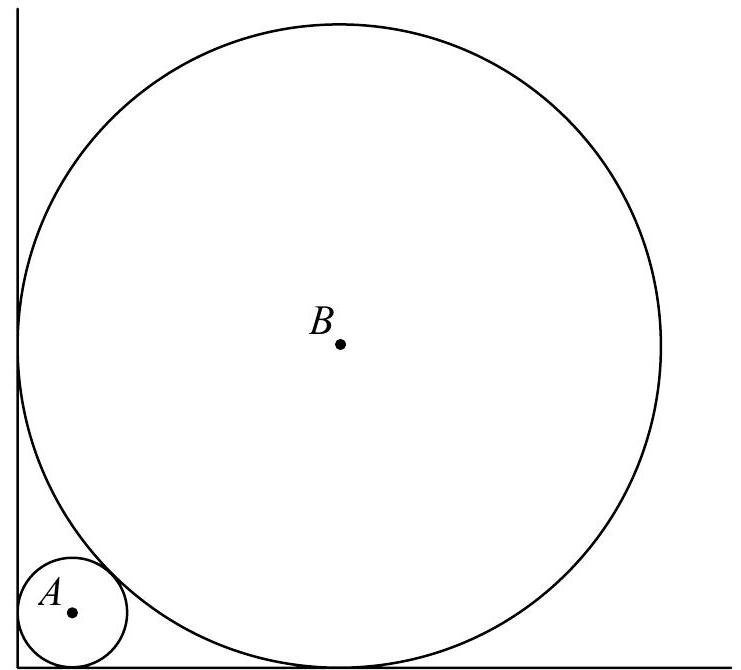
\includegraphics[max width=\textwidth, center]{2024_11_21_8bf32a7596bd08ca7a9fg-10}\\

\includegraphics[max width=\textwidth, center]{2024_11_21_8bf32a7596bd08ca7a9fg-10(1)}\\

\includegraphics[max width=\textwidth, center]{2024_11_21_8bf32a7596bd08ca7a9fg-11}

\begin{center}
\begin{tabular}{|c|l|c|c|c|c|}
\hline
\multirow{2}{*}{\begin{tabular}{c}
Wypełnia \\
egzaminator! \\
\end{tabular}} & Nr czynności & 8.1. & 8.2. & 8.3. & 8.4. \\
\cline { 2 - 6 }
 & Maks. liczba pkt & 1 & 1 & 1 & 1 \\
\cline { 2 - 6 }
 & Uzyskana liczba pkt &  &  &  &  \\
\hline
\end{tabular}
\end{center}

\section*{Zadanie 9. (5 pkt)}
W układzie współrzędnych narysuj okrag o równaniu \((x+2)^{2}+(y-3)^{2}=4\) oraz zaznacz punkt \(A=(0,-1)\). Prosta o równaniu \(x=0\) jest jedną ze stycznych do tego okręgu przechodzących przez punkt \(A\). Wyznacz równanie drugiej stycznej do tego okręgu, przechodzacej przez punkt \(A\).\\

\includegraphics[max width=\textwidth, center]{2024_11_21_8bf32a7596bd08ca7a9fg-12}

\begin{center}
\begin{tabular}{|c|l|c|c|c|c|c|}
\hline
\multirow{2}{*}{\begin{tabular}{c}
Wypetnia \\
egzaminator! \\
\end{tabular}} & Nr czynności & 9.1. & 9.2. & 9.3. & 9.4. & 9.5. \\
\cline { 2 - 7 }
 & Maks. liczba pkt & 1 & 1 & 1 & 1 & 1 \\
\cline { 2 - 7 }
 & Uzyskana liczba pkt &  &  &  &  &  \\
\hline
\end{tabular}
\end{center}

\section*{Zadanie 10. (4 pkt)}
W urnie znajdują się jedynie kule białe i czarne. Kul białych jest trzy razy więcej niż czarnych. Oblicz, ile jest kul w urnie, jeśli przy jednoczesnym losowaniu dwóch kul prawdopodobieństwo otrzymania kul o różnych kolorach jest większe od \(\frac{9}{22}\).\\

\includegraphics[max width=\textwidth, center]{2024_11_21_8bf32a7596bd08ca7a9fg-13}

\begin{center}
\begin{tabular}{|c|l|c|c|c|c|}
\hline
\multirow{2}{*}{\begin{tabular}{c}
Wypetnia \\
egzaminator! \\
\end{tabular}} & Nr czynności & 10.1. & 10.2. & 10.3. & 10.4. \\
\cline { 2 - 6 }
 & Maks. liczba pkt & 1 & 1 & 1 & 1 \\
\cline { 2 - 6 }
 & Uzyskana liczba pkt &  &  &  &  \\
\hline
\end{tabular}
\end{center}

\section*{Zadanie 11. (6 pkt)}
Dany jest ostrosłup prawidłowy trójkatny, w którym krawędź podstawy ma długość a i krawędź boczna jest od niej dwa razy dłuższa. Oblicz cosinus kąta między krawędzią boczna i krawędzią podstawy ostrosłupa. Narysuj przekrój ostrosłupa płaszczyzną przechodzaca przez krawędź podstawy i środek przeciwległej krawędzi bocznej i oblicz pole tego przekroju.\\
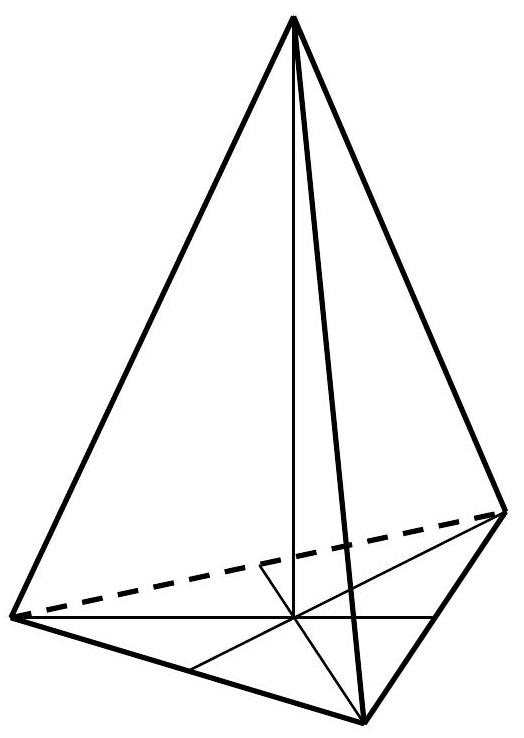
\includegraphics[max width=\textwidth, center]{2024_11_21_8bf32a7596bd08ca7a9fg-14}\\

\includegraphics[max width=\textwidth, center]{2024_11_21_8bf32a7596bd08ca7a9fg-14(1)}\\

\includegraphics[max width=\textwidth, center]{2024_11_21_8bf32a7596bd08ca7a9fg-15}

\begin{center}
\begin{tabular}{|c|l|c|c|c|c|c|c|}
\hline
\multirow{2}{*}{\begin{tabular}{c}
Wypełnia \\
egzaminator! \\
\end{tabular}} & Nr czynności & 11.1. & 11.2. & 11.3. & 11.4. & 11.5. & 11.6. \\
\cline { 2 - 8 }
 & Maks. liczba pkt & 1 & 1 & 1 & 1 & 1 & 1 \\
\cline { 2 - 8 }
 & Uzyskana liczba pkt &  &  &  &  &  &  \\
\hline
\end{tabular}
\end{center}

\section*{BRUDNOPIS}

\end{document}